\documentclass[12pt]{article}

\usepackage[utf8]{inputenc}
\usepackage[T1]{fontenc}
\usepackage[francais]{babel}
\usepackage{setspace}
\usepackage{bookman}
\usepackage{graphicx}
\usepackage{ulem}
\usepackage{url}
\usepackage{multicol}
\usepackage[top=1cm,left=1cm,right=1cm,bottom=2cm]{geometry}

\usepackage{vwcol}
\usepackage[hidelinks]{hyperref}


\begin{document}

\begin{figure}
	\centering
	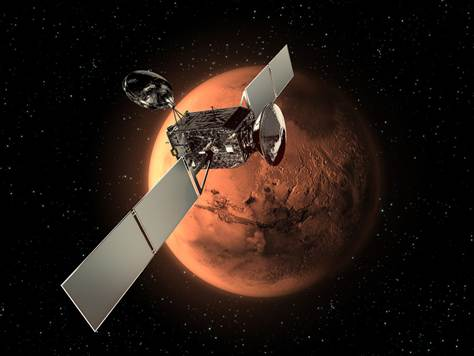
\includegraphics[scale=0.8]{images/logo.jpg}
\end{figure}

\hspace{\fill}

\begin{center}
	\LARGE{\textbf{Projet ExoLife}}
\end{center}


\begin{center}
\textbf{Analyse d'images pour but de trouver une source de vie dans l'univers, autre que sur Terre.}\\
\end{center}

\vspace{\fill}

\begin{flushright}
	\bsc{Chiaverini} Marie\\
	\bsc{Blochet} Tanguy\\
	\bsc{Saclier} Baptiste\\
\end{flushright}

\clearpage

\tableofcontents

\newpage

\section{Mission A}

	\subsection{Sous-Mission A1}

	
	
	\subsection{Sous-mission A2}

	\begin{vwcol}[widths={0.65,0.2}, rule=0pt]
		\begin{minipage}{0.7\textwidth}
			\paragraph{Objectifs de la mission}

			Déterminer la quantité de méthane dans l'atmosphère de la planète Mars, afin de déterminer si il y a une présence de vie sur cette planète. Pour se faire nous avions à disposition une photographie satellite de la surface de Mars.
		\end{minipage}

		\begin{minipage}{0.3\textwidth}
			\begin{flushright}
				\paragraph{Techniques utilisées}
			
				Proportion \&
				Moyenne
			\end{flushright}
		\end{minipage}
	\end{vwcol} 

	\begin{figure}[h]
	\centering
		
		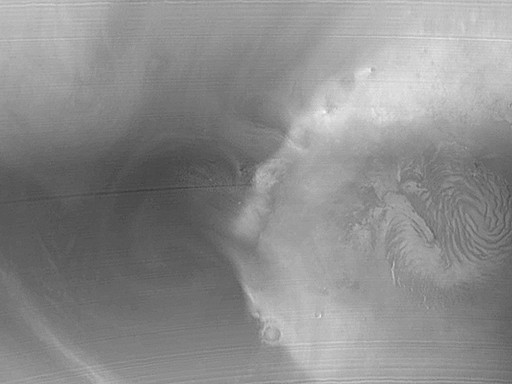
\includegraphics[scale=0.6]{images/Mars_surface.png}
		
	\end{figure}
	\vspace{-0.9cm}

	\paragraph{Procédé}	
		Pour remplir la mission nous avons calculé le taux de pixel, puis fais la somme des taux des pixels. Enfin, nous avons fait la moyenne du taux de gaz afin de déterminer la quantité de gaz dans l'atmosphère martienne. Nous n'avons pas eu besoin d'utiliser des filtres.

\newpage

	\subsection{Sous-mission A3}
	\subsection{Sous-mission A4}

	\begin{vwcol}[widths={0.8,0.2}, rule=0pt]
	\begin{minipage}{0.7\textwidth}
	\paragraph{Objectifs de la mission}

	Rendre une image de la planète Jupiter plus nette. Pour se faire nous avions à disposition deux photographies faites à quelques secondes d'intervalle comprenant toutes deux du bruit.
	\end{minipage}
	\begin{minipage}{0.2\textwidth}
	\paragraph{Filtres utilisés}

	\begin{itemize}
		\item Soustraction
		\item Filtre médiant
	\end{itemize}
	\end{minipage}
	\end{vwcol} 

	\begin{figure}[h]
	\centering
		\begin{multicols}{2}
		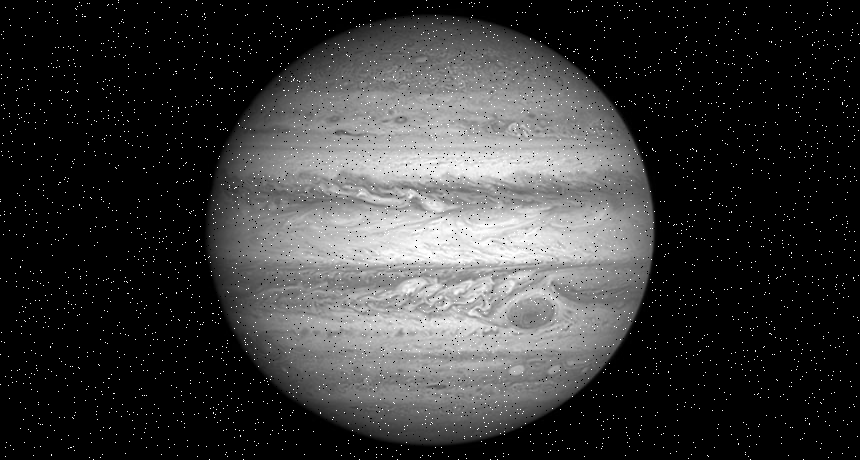
\includegraphics[scale=0.325]{images/Jupiter.png}
		Avant
		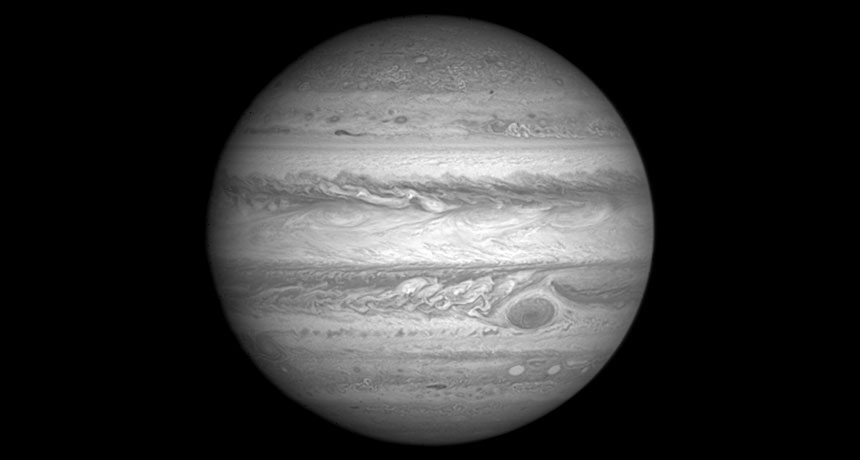
\includegraphics[scale=0.325]{images/JupiterAp.png}
		Après
		\end{multicols}
	\end{figure}
	\vspace{-0.9cm}

	\paragraph{Procédé}	
		Le résultat ci-dessus, nous avons utilisé deux filtes à la suite. Tout d'abord, nous avons \emph{soustrait} les deux images ensembles pour obtenir une troisième image ne comprenant que le bruit. Nous avons alors \emph{soustrait} ce résultat a l'image d'origine. Nous obtenons ensuite une image de meilleure qualité mais tout de même bruitée. Pour résoudre ce problème nous avons utilisé un \emph{filtre médiant} permettant de retirer le bruit sans altérer la netteté de l'image.

\newpage

\section{Mission B}
	\subsection{Sous-mission B1}

	\begin{vwcol}[widths={0.8,0.2}, rule=0pt]
	\begin{minipage}{0.7\textwidth}
	\paragraph{Objectifs de la mission}

	L'objectif de cette mission était de travailler l'image de Gliese 667Cc afin de faire apparaître son atmosphère sur les images prises par une sonde, cette image étant de mauvaise qualité. 
	\end{minipage}
	\begin{minipage}{0.2\textwidth}
	\paragraph{Filtre utilisé}

	\begin{itemize}
		\item Egalisation
	\end{itemize}
	\end{minipage}
	\end{vwcol} 

	\begin{figure}[h]
	\centering
		\begin{multicols}{2}
		
\includegraphics[scale=0.525]{images/Gliese667Cc.png}
		Avant
		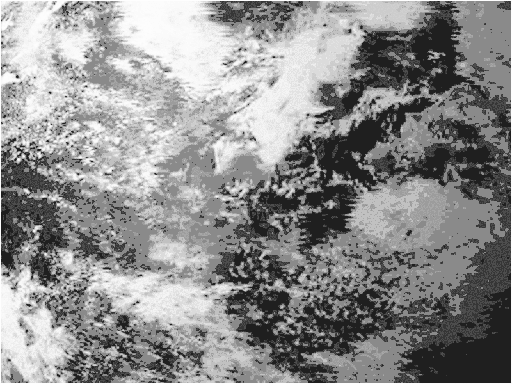
\includegraphics[scale=0.525]{images/Gliese667CcAFTER.png}
		Après
		\end{multicols}
	\end{figure}
	\vspace{-0.9cm}

		\paragraph{Procédé}	
			Pour cette mission une \emph{égalisation} a été réalisée sur cette image. Cette méthode fait nettement apparaître l'atmosphère de la planète. Une \emph{normalisation} avait été réalisée en premier lieu, qui faisait aussi apparaître cette atmosphère mais moins nettement.
		
\newpage

	\subsection{Sous-mission B2} 

	\begin{vwcol}[widths={0.8,0.2}, rule=0pt]
	\begin{minipage}{0.7\textwidth}
	\paragraph{Objectifs de la mission}

	L'objectif de cette mission était d'améliorer la visibilité de l'image afin de la donner à un autre service pour identifier la position d'une naine blanche située à 150 années lumière de la Terre.
	\end{minipage}
	\begin{minipage}{0.2\textwidth}
	\paragraph{Filtre utilisé}

	\begin{itemize}
		\item Normalisation
	\end{itemize}
	\end{minipage}
	\end{vwcol} 

	\begin{figure}[h]
	\centering
		\begin{multicols}{2}
		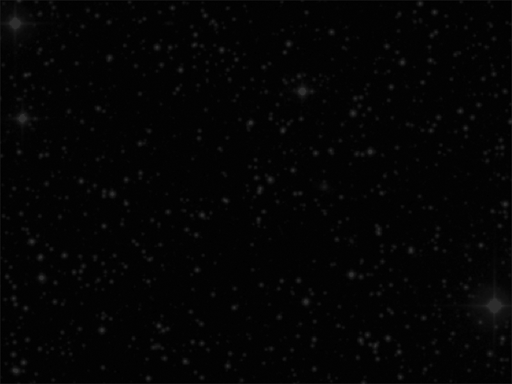
\includegraphics[scale=0.525]{images/GD61.png}
		Avant
		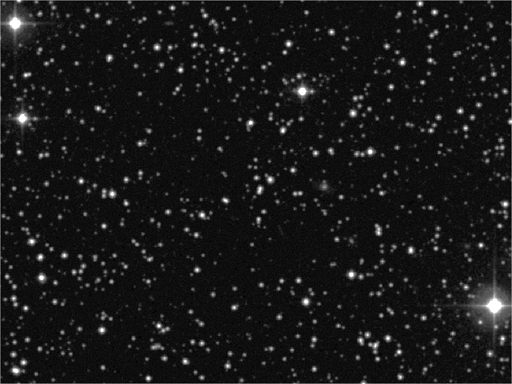
\includegraphics[scale=0.525]{images/GD61AFTER.png}
		Après
		\end{multicols}
	\end{figure}
	\vspace{-0.9cm}

		\paragraph{Procédé}	
			Pour cette mission une normalisation a été réalisée, faisant clairement apparaître les différentes planètes et étoiles.
		\par

\section{Mission X}

\section{Mission U}


\end{document}